\documentclass[11pt]{article}

% Packages
\usepackage[a4paper, margin=1in]{geometry}
\usepackage{amsmath, amssymb}
\usepackage{graphicx}
\usepackage{booktabs}
\usepackage{hyperref}
\usepackage{multirow}
\usepackage{float}
\usepackage{longtable}
\usepackage{xcolor}

\title{Cross-Sectional Equity Return Prediction using Machine Learning}
\author{Soham Tulsyan}
\date{\today}

\begin{document}

\maketitle

\begin{abstract}
Predicting equity returns is the "Holy Grail" of quantitative finance. This project aims to predict one-month forward equity returns using firm-level characteristics in a cross-sectional framework. We implement multiple machine learning models and evaluate them based on their ability to rank stocks using Information Coefficient (IC). Our findings highlight the effectiveness of factor-based features and ensemble methods in generating predictive signals. This report extends the mid-semester submission with completed implementations of the neural network module, ensemble layer, and a full portfolio backtesting analysis.
\end{abstract}

\section{Introduction}

\subsection{Motivation}
The central question that this project tries to examine is whether observable firm-level characteristics can predict future stock returns, or rather, systematically generate excess returns.
\subsubsection{The Efficient Market Hypothesis}
The Efficient Market Hypothesis (EMH) by Eugene Fama, posits that financial markets are informationally efficient, meaning asset prices at any given instant reflect all available information collated up to that point in time. Consequently, stocks always trade at their \textbf{fair} value, making it \textbf{impossible} for investors to consistently achieve returns exceeding average market returns on a risk-adjusted basis.

There are three forms to this hypothesis:
\begin{itemize}
    \item \textbf{The Weak Form} suggests that all past trading information regarding prices and volume is already reflected in current prices, meaning technical analysis cannot produce superior returns.
    \item \textbf{The Semi-Strong Form} suggests that all publicly available information including financial statements, news, and analyst reports is already reflected in current prices, meaning fundamental analysis cannot produce superior returns.
    \item \textbf{The Strong Form} suggests that all information, both public and private, is already reflected in current prices, meaning no investor can produce superior returns.
\end{itemize}
This hypothesis forms a foundation for modern finance, however, is widely debated. In our project, we aim to challenge this hypothesis - particularly the semi-strong form - by predicting future stock returns using firm-level characteristics.

\subsubsection{Factor Investing}
Factor investing is a data-driven investment strategy that selects securities based on specific company-level characteristics("factors") associated withs higher returns, such as value, quality, momentum, and low volatility. It acts as a hybrid between active and passive investing, using systematic, rules-based approaches to enhance diversification and target higher risk-adjusted returns.

Factor investing, in essence, contradicts the EMH, and forms the basis of this project, where we analyse the predictive power of various company level factors on future stock returns.

\subsection{Objective}
Building on the theoretical foundations of Factor Investing, our objective is to develop a systematic, data-driven framework for evaluating return predictability in financial markets. Specifically, we focus on applying statistical and machine learning techniques to cross-sectional equity data in order to identify, quantify, and validate predictive signals embedded in firm-level characteristics. Emphasis is placed not only on model construction, but also on rigorous evaluation using economically meaningful metrics, ensuring that any detected patterns translate into robust and implementable investment strategies.

\subsection{Hypothesis}

Our hypothesis can be stated as a combination of the following points:

\begin{itemize}
    \item Firm-level characteristics, such as value, size, profitability, investment, and momentum, contain statistically significant information for predicting cross-sectional differences in future stock returns.

    \item Non-linear machine learning models are better suited to capture complex interactions and non-linear relationships among these factors compared to traditional linear models, leading to improved predictive performance.

    \item Ensemble methods, by combining multiple models, can further enhance predictive accuracy and robustness relative to individual model approaches.
\end{itemize}

We must design our pipeline and structure in a way that allows us to systematically test these hypotheses, and evaluate the performance of each model using economically meaningful metrics. More on this in the methodology section.

\subsection{Goals}
To put our project into action and test our ideas, we have set the following practical goals and milestones for our pipeline:

\begin{itemize}
    \item \textbf{Cleaning and Preparing the Data}: To build a clean, 25-year dataset of US stocks (2001--2025). We need to make sure factors like Size and Value are scaled properly and that there is absolutely no look-ahead bias in our data.
    \item \textbf{Building a Realistic Test Engine}: To create a "walk-forward" testing system that mimics how an actual trader sees the market - moving forward one month at a time and only using information available at that moment.
    \item \textbf{Comparing Simple vs. Complex Models}: To see if complex models like LightGBM and Random Forest actually perform better than a simple linear model like Ridge. This helps us decide if the extra complexity is worth the effort.
    \item \textbf{Setting up a Quality-Control System}: To regularly check our model's "health" using stats like IC (to see if we're actually predictive) and VIF (to make sure our factors aren't just overlapping).
    \item \textbf{Developing an Investable Portfolio}: Our ultimate goal is to turn these rankings into a real-world long-short portfolio. We want to see if we can identify the best and worst stocks to potentially trade them in the real market.
\end{itemize}


\section{Methodology}

\subsection{Checklist}
To test the validity of each of our hypotheses, we follow the following layered pipeline structure:

\begin{enumerate}
    \item To test the first part of our hypothesis, we must first set a linear baseline. We use simple linear models to derive a meaningful and statistically significant correlation between our factors and future stock returns. For this, we will be using Linear Ridge Regression. If we are successful at deriving a statistically significant correlation, it would mean that our factors have some predictive power. Thus, even if the accuracy is low, we can proceed further.
    \item To test the second part of our hypothesis, we can introduce a tri-moduled structure. Essentially, this layer can be divided into a \textbf{Tree Module}, a \textbf{Neural Network Module}, and an \textbf{Random Forest Module}. Each of these modules approaches the problem of non-linearity slightly differently, and can be compared across both a linear and a non-linear baseline. If non-linearity provides better results, then we can conclude the validity of the second part of our hypothesis. If any models perform worse than the linear baseline, we can deem them exceptions and proceed with added complexity, however, if this seems to be the general trend in this layer, then our hypothesis fails.
    \item Finally, to address the third part of our hypothesis, we can form an ensemble of the best models from the previous layers to see if we can further improve the predictive accuracy and robustness of our model. However, if the added complexity does not result in significant improvements compared to the benchmarks set by the previous layers, then we opt for the simplicity of a Layer 2 or Layer 1 model.
\end{enumerate}

\subsection{Problem Setup}
At each time step (which, in this case, is a month) \( t \), we predict returns at \( t+1 \) for all firms. This is a panel data problem with both time-series and cross-sectional dimensions. We will be using a walk-forward validation approach to evaluate the performance of our models. Future improvements can address time-series characteristics, however, as for now, we will be treating each month as an independent cross-section.

\subsection{Data Description}

The dataset used in this study is obtained from the \href{https://jkpfactors.s3.amazonaws.com/documents/Documentation.pdf}{JKP Factors dataset}. It consists of firm-level monthly panel data, where each row corresponds to a firm (\texttt{co\_code}) at a given month (\texttt{Month}).

\subsubsection{Dataset Schema}

\begin{table}[H]
\centering
\small
\begin{tabular}{|l|l|p{7cm}|}
\hline
\textbf{Category} & \textbf{Variable} & \textbf{Description} \\
\hline

Identifiers & co\_code & Unique firm identifier \\
Identifiers & Month & Observation month (YYYY-MM format) \\
Identifiers & Year & Calendar year of observation \\

\hline
Target & monthly\_gross\_return & Monthly stock return (next-period prediction target) \\

\hline
Value & BM\_sep & Book-to-market ratio \\

\hline
Size & lag\_mv & Lagged market value (firm size proxy) \\

\hline
Profitability & OpProf & Operating profitability derived from accounting variables \\

\hline
Investment & Inv & Asset growth rate (investment measure) \\

\hline
Momentum / Returns & Momentum & 12--1 momentum signal \\
Momentum / Returns & lag\_ret & Lagged return (short-term reversal) \\
Momentum / Returns & log\_ret & Log-transformed return \\

\hline
Accounting Variables & sa\_sales & Total sales \\
Accounting Variables & sa\_cost\_of\_goods\_sold & Cost of goods sold \\
Accounting Variables & sa\_total\_interest\_exp & Interest expenses \\
Accounting Variables & sa\_selling\_distribution\_exp & Selling and distribution expenses \\
Accounting Variables & lagged\_book\_equity & Lagged book equity \\
Accounting Variables & lagged\_assets & Lagged total assets \\

\hline
Market Variables & price & Stock price \\
Market Variables & mktcap & Market capitalization (excluded due to leakage concerns) \\

\hline
Categorical Labels & Size\_Label & Size-based grouping \\
Categorical Labels & BM\_Label & Value-based grouping \\
Categorical Labels & OpProf\_Label & Profitability grouping \\
Categorical Labels & Inv\_Label & Investment grouping \\
Categorical Labels & Mom\_Label & Momentum grouping \\

\hline
\end{tabular}
\caption{Summary of dataset variables and their economic interpretation}
\end{table}

\subsection{Data Preprocessing}

To ensure consistency with the cross-sectional prediction framework and to avoid any form of look-ahead bias, the dataset undergoes the following preprocessing steps:

\subsubsection{Data Ordering}

The dataset is first sorted by firm and time:
\begin{itemize}
    \item Sort by \texttt{co\_code} and \texttt{Month}
\end{itemize}
This ensures correct temporal alignment when constructing lagged features and forward returns.

\subsubsection{Forward Return Construction}

The prediction target is defined as the next-period return:
\begin{itemize}
    \item \texttt{monthly\_gross\_return} at time $t+1$ is assigned to features at time $t$
\end{itemize}
This step ensures that all predictions are strictly out-of-sample and prevents information leakage.

\subsubsection{Feature Selection}

Only economically motivated factors are retained for model training:
\begin{itemize}
    \item \texttt{BM\_sep} (Value)
    \item \texttt{lag\_mv} (Size)
    \item \texttt{OpProf} (Profitability)
    \item \texttt{Inv} (Investment)
    \item \texttt{Momentum} (12--1 momentum)
    \item \texttt{lag\_ret} (Short-term reversal)
    \item \texttt{mktcap} (Log-transformed size)
\end{itemize}

The variable \texttt{mktcap} is included in our feature set; however, its use requires a significant note of caution to prevent data leakage. Market capitalization is defined as:
\[
\texttt{mktcap}_t = \texttt{price}_t \times \texttt{shares\_outstanding}_t
\]

Since stock returns are directly driven by changes in price, we have:
\[
\text{return}_{t+1} \approx \frac{\texttt{price}_{t+1}}{\texttt{price}_t} - 1
\]

This implies that \texttt{mktcap} at time $t$ is closely tied to $\texttt{price}_t$. If not handled with care, it can inadvertently encode the realized return of the current period. Specifically, the relationship $\frac{\texttt{mktcap}_t}{\texttt{mktcap}_{t-1}} \approx 1 + \text{return}_t$ could allow a model to reconstruct the very returns it is meant to predict. To mitigate this risk and ensure strict out-of-sample integrity, we implement the following safeguards:

\begin{itemize}
    \item \textbf{Strict Lagging}: All features, including \texttt{mktcap}, are strictly lagged by one month. Thus, we only use information finalized at $t-1$ to predict the return at $t$.
    \item \textbf{Log-Transformation}: As market capitalization often follows a power-law distribution and exhibits high skewness, we apply a log-transform ($\ln(1 + x)$) to normalize the distribution and limit the influence of extreme values.
    \item \textbf{Rank Normalization}: In the machine learning pipelines, we replace raw values with cross-sectional ranks, ensuring the "size" signal is based on the relative position of the firm within the universe rather than absolute price levels.
\end{itemize}

By applying these safeguards, we retain the predictive power of the size factor while insulating the model from the risk of mechanical look-ahead bias.

\subsubsection{Null Handling}

Observations with missing values in either features or the target variable are removed, i.e, all rows with 'N/A' values are dropped.
This ensures a consistent cross-sectional sample at each time step.

\subsubsection{Outlier Treatment via Winsorization}

Financial datasets are often characterized by extreme values due to market shocks, data errors, or illiquid stocks. Such outliers can disproportionately influence model estimation, especially for machine learning models that are sensitive to the scale and distribution of input features.

To mitigate this issue, we apply \textbf{winsorization} to all continuous features.

Winsorization is a transformation that limits extreme values by capping them at specified percentile thresholds, rather than removing them entirely. Specifically, for each feature and for each month, values are adjusted as follows:
\begin{itemize}
    \item Values below the 1st percentile are set equal to the 1st percentile
    \item Values above the 99th percentile are set equal to the 99th percentile
\end{itemize}

Formally, for a variable $x_{i,t}$:
\[
x^{\text{wins}}_{i,t} =
\begin{cases}
P_{1,t} & \text{if } x_{i,t} < P_{1,t} \\
x_{i,t} & \text{if } P_{1,t} \leq x_{i,t} \leq P_{99,t} \\
P_{99,t} & \text{if } x_{i,t} > P_{99,t}
\end{cases}
\]
where $P_{1,t}$ and $P_{99,t}$ denote the 1st and 99th percentiles of the cross-sectional distribution at time $t$.

This approach preserves the majority of the data while reducing the influence of extreme observations, leading to more stable and robust model estimates. Importantly, winsorization is preferred over outright removal of outliers, as it maintains the cross-sectional structure of the dataset, which is critical for ranking-based evaluation.

\subsubsection{Cross-Sectional Normalization}

Since the objective is to predict relative rankings, all features and the target are normalized cross-sectionally:

For each month, transform variables into z-scores:
    \[
    z_{i,t} = \frac{x_{i,t} - \mu_t}{\sigma_t}
    \]
where $\mu_t$ and $\sigma_t$ are the cross-sectional mean and standard deviation at time $t$

This ensures comparability across time and aligns the data with rank-based evaluation metrics such as the Information Coefficient (IC).

\subsubsection{Final Dataset Construction}

After preprocessing:
\begin{itemize}
    \item Each observation corresponds to $(i, t)$ with features at time $t$
    \item Target corresponds to return at time $t+1$
    \item Data is ready for walk-forward validation
\end{itemize}


To evaluate the models' performance realistically and ensure no look-ahead bias, we employ a \textbf{Walk-Forward Validation} (sliding window) approach. This method mimics a real-world investment process where a model is trained on available historical data and tested on the immediate following period.

\begin{itemize}
    \item \textbf{Training Window}: For the machine learning models (Random Forest and LightGBM), we use a rolling window of 60 months (5 years) of historical data for each training fold.
    \item \textbf{Walk-Forward Mechanism}: The window slides forward by one month at a time. For each month $t$, the model is trained on the period $[t-60, t-1]$ and generates predictions for the cross-section of stocks in month $t$.
    \item \textbf{Consistency}: This process is repeated across the entire dataset (May 2001 -- March 2025), resulting in a time-series of monthly Information Coefficients (IC) that measures the stability and reliability of the alpha across different market regimes.
\end{itemize}

\section{Pipeline}
As previously discussed, we use a multi-layered comparison based pipeline, where each layer adds complexity to our overall model.
\subsection{Pipeline Diagram}
\begin{figure}[!htb]
    \centering
    
\includegraphics[width=\textwidth, height=0.88\textheight, keepaspectratio]{Pipeline Diagram.png}
    \caption{Full pipeline architecture, from raw data through the linear baseline, non-linear layer, ensemble, portfolio construction, and the proposed reinforcement learning extension.}
    \label{fig:pipeline}
\end{figure}

\subsection{Layer 1: Linear Baseline}
In the first layer of our pipeline, we implement a linear factor model to establish a performance baseline. This allows us to determine if complex machine learning models actually add value beyond standard linear relationships. It also allows us to assess the first part of our hypothesis, as discussed earlier.

\subsubsection{Ridge Regression}
Ridge Regression serves as our fundamental linear benchmark. \[
r_{i,t+1} = \beta_{0,t} + \beta_{1,t} \text{BM\_sep}_{i,t} + \beta_{2,t} \text{OpProf}_{i,t} + \beta_{3,t} \text{Inv}_{i,t} + \beta_{4,t} \text{Momentum}_{i,t} + \beta_{5,t} \text{lag\_ret}_{i,t} + \beta_{6,t} \text{mktcap}_{i,t} + \epsilon_{i,t+1}
\]
where $r_{i,t+1}$ is the excess return of stock $i$ in month $t+1$, and the features represent the six primary signals (Value, Profitability, Investment, Momentum, Short-term Reversal, and Size) observed at time $t$. To estimate the coefficients $\beta_{k,t}$, Ridge extends standard Ordinary Least Squares (OLS) by adding an $L2$ penalty term to the cost function:
\[
\min_{w} ||Xw - y||^2_2 + \alpha ||w||^2_2
\]
This regularization is critical in our context, as firm-level factors (like size and value) often exhibit high multicollinearity, which can make OLS estimates unstable. Ridge Regression allows us to mitigate this issue by shrinking the coefficients towards zero, effectively reducing the impact of multicollinearity.

Our implementation follows a rigorous monthly pipeline:

\begin{itemize}
    \item \textbf{Dynamic Hyperparameter Tuning}: The optimal regularization strength $\alpha$ is selected every month using time-series cross-validation on the training cross-section.
    \item \textbf{Assumption Validation}: We perform extensive diagnostics including \textbf{Pre-checks} for feature variance and Multicollinearity (VIF). After estimation, \textbf{Post-checks} are conducted on residuals to monitor Normality (Jarque-Bera), Homoscedasticity (Breusch-Pagan), and Autocorrelation (Durbin-Watson).
    \item \textbf{Standardized Importance}: features are cross-sectionally standardized to allow for a direct comparison of factor coefficients across different regimes.
\end{itemize}

\subsection{Layer 2: Non-Linear Layer}
As mentioned before, the 2nd Layer consists of a tri-modular structure, each module consisting of different forms of non-linear models. The modules are enumerated below:
\subsubsection{Tree Module}
This module serves as the sort of a baseline for non-linear models. The module consists of 2 models: \textbf{CART} (specifically, Regression Trees) and \textbf{LightGBM}.
\begin{itemize}
    \item \textbf{CART (Classification and Regression Trees)}:
    As a baseline for non-linear models, we implement a Regression Tree to capture simple non-linear interactions and threshold effects. The model follows a recursive binary partitioning process. At each node, the optimal feature $j$ and splitting threshold $\tau$ are identified by minimizing the weighted Mean Squared Error (MSE):
    \[
    \underset{j, \tau}{\arg\min} \left[ \frac{|R_L|}{n} \text{MSE}(R_L) + \frac{|R_R|}{n} \text{MSE}(R_R) \right]
    \]
    where $R_L = \{x : x_j \leq \tau\}$ and $R_R = \{x : x_j > \tau\}$. For a given terminal leaf node $R_m$, the predicted return $\hat{y}$ is the mean of all training observations within that partition:
    \[
    \hat{y} = \frac{1}{|R_m|} \sum_{i \in R_m} y_i
    \]

    To prevent overfitting and ensure generalization, we utilize \textbf{Cost-Complexity Pruning}, which selects the subtree $T_\alpha$ that minimizes the penalized objective:
    \[
    C_\alpha(T) = \sum_{m=1}^{|T|} \text{MSE}(R_m) + \alpha \cdot |T|
    \]
    where $|T|$ represents the number of terminal nodes and $\alpha$ is a complexity parameter that penalizes larger trees. Finally, we assess factor relevance using \textbf{Mean Decrease in Impurity (MDI)}:
    \[
    \text{Importance}(j) = \sum_{\text{nodes } t \text{ split on } j} \frac{n_t}{n} \left[ \text{MSE}(t) - \frac{n_L}{n_t}\text{MSE}(t_L) - \frac{n_R}{n_t}\text{MSE}(t_R) \right]
    \]
    \begin{itemize}
        \item \textbf{Feature Set}: Identical to the Ridge baseline, incorporating \texttt{BM\_sep}, \texttt{OpProf}, \texttt{Inv}, \texttt{Momentum}, \texttt{lag\_ret}, and \texttt{mktcap}.
        \item \textbf{Regularization and Tuning}: To prevent overfitting, we tune key tree hyperparameters, including the maximum depth (\texttt{max\_depth} $\in \{3, 5, 10\}$) and the minimum number of observations per leaf (\texttt{min\_samples\_leaf} $\in \{5, 10, \dots, 50, 100\}$).  Hyperparameter selection is performed using a grid search over the specified parameter space. Each candidate configuration is evaluated using a rolling one-step-ahead validation scheme, where the model is trained on data from month $t$ and tested on month $t+1$. Model performance is assessed using the Information Coefficient (IC), and the configuration with the highest risk-adjusted performance (ICIR) is selected.
        \item \textbf{Implementation Note}: Our current implementation utilizes a \textbf{one-month walk-forward validation} (training on month $t$ to predict $t+1$). While this ensures perfect temporal integrity, the single-month training sample may be sensitive to idiosyncratic noise and market volatility. We acknowledge this as a limitation and plan to expand the training window to a larger rolling format in subsequent research iterations to more effectively capture long-term factor distributions.
    \end{itemize}
    \item \textbf{LightGBM (Light Gradient Boosting Machine): }
    LightGBM is a high-performance gradient boosting framework that uses tree-based learning algorithms. It is specifically optimized for speed and memory efficiency on large-scale financial panel data. Unlike standard gradient boosting trees that grow level-wise, LightGBM grows trees \textit{leaf-wise}. This approach allows it to achieve lower loss and higher accuracy in capturing complex, non-linear relationships, though it necessitates rigorous hyperparameter tuning to mitigate overfitting.

    Our pipeline implements several advanced safeguards to maximize the model's predictive power:
    \begin{itemize}
        \item \textbf{Cross-Sectional Rank-Normalization}: To handle outliers and the changing scale of economic factors across different market regimes, we transform our features into cross-sectional percentile ranks ($[0,1]$) within each month. This focusing ensure the model's objective is the relative ordering of stocks.
        \item \textbf{Rolling Window Training}: Unlike the baseline CART model, the LightGBM pipeline utilizes a \textbf{60-month (5-year) rolling training window}. This provides a larger sample size to capture stable cross-sectional relationships while sliding forward to keep the model updated with the latest market dynamics. Though, inadvertently, this gives the LightGBM pipeline a significant advantage over our CART implementation, our aim with CART was to serve as a baseline that we compare more complex models to. A single regression tree is very prone to overfitting, which is why it is not being considered in our ensemble.
        \item \textbf{Hyperparameter Optimization}: We implement an extensive grid search to optimize key parameters, including the learning rate, the number of leaves, and the tree depth. These are selected to maximize the risk-adjusted Information Coefficient (ICIR) over an initial validation period.
        \item \textbf{Diagnostic Audits}: The pipeline performs a continuous \textbf{leakage audit} to ensure that lagged features do not inadvertently contain future information. Post-estimation, we generate aggregate feature importance scores to quantify the economic contribution of each factor over time.
    \end{itemize}
\end{itemize}
\subsubsection{Random Forest Module}
This module consists mainly of a \textbf{Random Forest} model, which is an ensemble of multiple regression trees.
\\
\\
The Random Forest model is created as follows:

\begin{itemize}
    \item \textbf{Bootstrap Aggregation (Bagging)}: The model constructs a large ensemble of independent regression trees, each trained on a different bootstrap sample (sampling with replacement) of the 60-month training window. By averaging the predictions across these trees, we significantly reduce the ensemble's variance and avoid the overfitting problems inherent in a single decision tree.
    \item \textbf{Feature Randomization}: To further decorrelate the individual trees, we limit the number of features considered at each node split. Our pipeline tunes this (\texttt{max\_features}) between a square-root rule and a 50\% subset rule to optimize the tradeoff between the individual tree's predictive power and the overall ensemble's diversity.
    \item \textbf{Rank-Based Prediction}: Consistent with the LightGBM module, all features are converted to cross-sectional percentile ranks ($[0,1]$) within each month. This ensures that the Random Forest focuses on identifying the \textit{relative positioning} of returns rather than being biased by absolute magnitudes or non-Gaussian returns.
    \item \textbf{Ensemble Optimization}: We employ a parallelized grid search to select the optimal forest architecture, including the number of trees (\texttt{n\_estimators}) and the minimum leaf size (\texttt{min\_samples\_leaf}), ensuring the model is robust enough to generalize across different market regimes.
\end{itemize}
\subsubsection{Neural Network Module}
This module addresses complex non-linear relationships that may arise in the data. We implement two architectures: a \textbf{Multi-Layer Perceptron (MLP)} as our baseline and a \textbf{Transformer} as a more expressive alternative.

\textbf{Multi-Layer Perceptron (MLP):} The MLP is a standard feed-forward neural network trained on the same cross-sectional rank-normalized features used throughout the pipeline. The architecture uses two hidden layers with ReLU activations and batch normalization, along with dropout regularization and early stopping to prevent overfitting on the relatively small monthly cross-sections. The model is retrained monthly on the 60-month rolling window, consistent with the tree-based ensembles. The objective is to minimize the mean squared error between predicted and realized returns, with the final ranking derived from the predicted values.

\textbf{Transformer:} The Transformer was adapted from its original sequence-to-sequence formulation to a cross-sectional ranking problem. Each stock in a given month is treated as a token, and the self-attention mechanism learns pairwise relationships between stocks in the same cross-section. This allows the model to capture group-level dynamics, such as sector rotation or broad factor tilts, that a per-stock prediction approach would miss entirely. The model uses a small number of attention heads to keep the capacity in check, given the limited number of training samples available each month.

\subsection{Layer 3: The Ensemble Layer}
This layer will essentially serve to combine the results of the previous 2 layers, to produce a potentially more refined result. Something to note here is that we will not necessarily be using all the models from the previous layers. We compare each model to the baselines that we have set, and only include those models which significantly surpass this threshold.

We have 2 ways of going about this:
\begin{itemize}
    \item A simple average of the predictions from the previous models. This weighs each model equally, no matter how much better any one of them might. We will use this as our baseline for the Ensemble Layer.
    \item An optimally weighted average derived from a 'Meta-Learner' model:\\
    \\
    The meta-learner is a Ridge regression that learns a weight for each Layer 1 and 2 model:

$$\hat{y}_{final}(i,t) = \alpha + w_1 \hat{y}_{ridge} + w_2 \hat{y}_{cart} + w_3 \hat{y}_{lgbm} + w_4 \hat{y}_{rf} + w_5 \hat{y}_{mlp} + w_6 \hat{y}_{transformer}$$

Based on our level of 'trust' on each model - which is essentially a measure of how good an output each model produced, this Meta Learner can allot optimal weights and give us the final prediction. \\
\\
A few things to note about the choice of the Meta-Learner are that firstly, we opt for a Ridge Regression over a simple Linear Regression, as the predictions from the Layer 1 and 2 models may be very highly correlated (e.g. LightGBM and Random Forest often identify the same alpha signals). Ridge handles this multi-collinearity by shrinking coefficients, leading to a more stable and balanced trust weight across models.

    Additionally, the Meta-Learner is strictly trained on the outputs rather than the raw economic factors, serving as an "unbiased judge" of the previous layers.
\end{itemize}

\subsubsection{Stacked Generalization}
The most critical implementation detail for this layer is the prevention of data leakage through \textbf{Stacked Generalization}. To ensure the meta-learner generalizes correctly, it is trained using \textbf{Out-of-Fold (OOF) Predictions}.

\begin{itemize}
    \item \textbf{Leakage Prevention}: We avoid training the meta-learner on the base models' standard training predictions. Doing so would lead to overfitting, as the meta-learner would naturally over-index on models that overfitted the training set.
    \item \textbf{K-Fold Methodology}: We split the training dataset into 5 folds. For each fold $k$, we train the base models on the other 4 folds and generate predictions for fold $k$. These stacked OOF predictions (shaped $N_{stocks} \times N_{models}$) form the true training set for the meta-learner.
\end{itemize}

\subsubsection{Full Training and Inference Flow}
Our ensemble pipeline follows a strict multi-step sequence:
\begin{enumerate}
    \item \textbf{OOF Generation}: Use 5-fold CV on the training set to collect unbiased predictions for all base models.
    \item \textbf{Meta-Training}: Train the Meta-Learner (Ridge) on these OOF predictions against the actual returns.
    \item \textbf{Model Retraining}: Retrain all base models (Ridge, CART, LGBM, RF, MLP, Transformer) on the full training dataset to maximize their predictive power.
    \item \textbf{Final Inference}: On the test set, each base model predicts a return; these are passed through the meta-learner to produce the final ranking $\hat{y}_{final}$.
    \item \textbf{Evaluation}: Compute IC and ICIR on the final refined predictions to measure alpha stability.
\end{enumerate}

\section{Evaluation}

Evaluating predictive performance in a financial context requires a framework that aligns with the ultimate objective of the model, namely, \textit{ranking stocks by expected returns} rather than accurately predicting return magnitudes. Accordingly, we adopt evaluation metrics and validation procedures that are consistent with cross-sectional asset pricing and portfolio construction.

\subsubsection{Information Coefficient (IC)}

The primary metric used in this study is the \textbf{Information Coefficient (IC)}, defined as the Spearman rank correlation between predicted returns and realized returns in each month:

\[
IC_t = \text{Spearman}(\hat{r}_{i,t}, r_{i,t})
\]

where $\hat{r}_{i,t}$ denotes the predicted return for stock $i$ at time $t$, and $r_{i,t}$ denotes the realized return.

The IC measures the model's ability to correctly rank stocks in a cross-section. A positive IC indicates that stocks predicted to perform well tend to outperform those predicted to perform poorly.

\paragraph{Interpretation}
\begin{itemize}
    \item $IC > 0$: Model has predictive power
    \item $IC \approx 0$: No predictive signal
    \item $IC < 0$: Inverse signal (potentially exploitable)
\end{itemize}

Rather than evaluating performance at a single point in time, we compute a time series of monthly IC values and summarize them using:
\begin{itemize}
    \item Mean IC
    \item Standard deviation of IC
    \item Percentage of months with positive IC
\end{itemize}

\subsubsection{Information Coefficient Information Ratio (ICIR)}

To assess the \textit{consistency} of predictive performance, we compute the \textbf{Information Coefficient Information Ratio (ICIR)}:

\[
ICIR = \frac{\mathbb{E}[IC_t]}{\sigma(IC_t)}
\]

The ICIR measures the stability of the signal over time, analogous to a Sharpe ratio for predictive accuracy.

\paragraph{Interpretation}
\begin{itemize}
    \item Higher ICIR indicates more stable and reliable predictions
    \item A model with moderate IC but high ICIR may be preferable to one with volatile performance
\end{itemize}

\subsubsection{Why Not RMSE or $R^2$?}

Traditional regression metrics such as Mean Squared Error (MSE), Root Mean Squared Error (RMSE), and $R^2$ are not well-suited for this problem due to the following reasons:

\begin{itemize}
    \item \textbf{Objective mismatch}: These metrics evaluate the accuracy of predicted return magnitudes, whereas our objective is to correctly rank stocks in the cross-section.

    \item \textbf{Low signal-to-noise ratio}: Equity returns are highly noisy and difficult to predict in levels. A model may have poor RMSE but still correctly rank stocks, which is sufficient for profitable portfolio construction.

    \item \textbf{Scale sensitivity}: MSE-based metrics are sensitive to extreme values and outliers, which are common in financial data.

    \item \textbf{Economic irrelevance}: A model that minimizes RMSE does not necessarily produce a profitable trading strategy, whereas a model with positive IC can be directly translated into an investment signal.
\end{itemize}

Thus, IC-based evaluation provides a more appropriate measure of model performance in the context of cross-sectional return prediction.

\subsubsection{Walk-Forward Evaluation Procedure}

To ensure realistic and unbiased evaluation, we employ a walk-forward validation framework:

\begin{itemize}
    \item Train the model on a rolling window of the past 60 months
    \item Generate predictions for month $t+1$
    \item Compute IC for that month
    \item Slide the window forward and repeat
\end{itemize}

This produces a time series of out-of-sample IC values, which forms the basis of all evaluation metrics.

\subsubsection{Economic Evaluation via Portfolio Construction}

While statistical metrics such as IC provide insight into predictive accuracy, it is essential to evaluate whether the model generates economically meaningful returns. To this end, we construct a long-short portfolio based on model predictions.

\paragraph{Portfolio Formation}

For each month:
\begin{itemize}
    \item Rank all stocks based on predicted returns
    \item Form quantile portfolios (deciles)
    \item Go \textbf{long} on the top decile (highest predicted returns)
    \item Go \textbf{short} on the bottom decile (lowest predicted returns)
\end{itemize}

The long-short portfolio return is computed as:

\[
R_t^{LS} = \frac{1}{N_{top}} \sum_{i \in \text{Top}} r_{i,t}
- \frac{1}{N_{bottom}} \sum_{i \in \text{Bottom}} r_{i,t}
\]

This represents a zero-investment strategy that isolates the model's predictive signal.

\paragraph{Performance Metrics}

We evaluate the portfolio using:
\begin{itemize}
    \item Mean return
    \item Volatility
    \item Sharpe ratio
\end{itemize}

\paragraph{Interpretation}

A consistently positive long-short return indicates that the model successfully identifies mispriced securities and that the predictive signal is economically exploitable.

\subsubsection{Summary}

The evaluation framework combines:
\begin{itemize}
    \item \textbf{Statistical validation} via IC and ICIR
    \item \textbf{Robust out-of-sample testing} via walk-forward validation
    \item \textbf{Economic validation} via portfolio backtesting
\end{itemize}

This ensures that model performance is assessed not only in terms of predictive accuracy but also in terms of real-world investment applicability.
\section{Evaluation}
\subsection{Benchmarks}
To provide context for the performance of our models, we adopt several standardized benchmarks used in quantitative finance and asset pricing literature.

\subsubsection{Statistical Thresholds (IC and ICIR)}
We use the following thresholds to interpret the strength and stability of our model signals:

\begin{table}[H]
\centering
\begin{tabular}{ll}
\toprule
\textbf{ICIR Range} & \textbf{Interpretation} \\
\midrule
$< 0.2$   & Noise / Weak Signal \\
0.3 -- 0.5 & Moderate Signal \\
0.5 -- 1.0 & Good Predictive Signal \\
$> 1.0$    & Strong / Significant Signal \\
\bottomrule
\end{tabular}
\caption{Standard interpretation of the IC Information Ratio (ICIR).}
\end{table}

Specifically, an Information Coefficient (IC) greater than \textbf{0.03} sustained over a long-term walk-forward period is considered evidence of a genuinely predictive and robust factor in academic literature.

\subsubsection{Economic Threshold (Sharpe Ratio)}
From an implementation perspective, we evaluate the profitability of our long-short portfolios. An investment strategy is generally considered "economically viable" or implementable in practice if it achieves an annualized \textbf{Sharpe ratio greater than 0.8}, indicating that the returns are sufficient to compensate for risk and transaction costs.

\section{Results}

% =====================================================================
% NOTE: The Ridge, CART, LightGBM, and Random Forest sections below
% were presented at the mid-semester checkpoint. The subsequent sections
% (MLP, Transformer, Ensemble, and Portfolio Testing) represent work
% completed after the mid-semester presentation.
% =====================================================================

\subsection{Ridge Regression Baseline Results}
The Ridge Regression model establishes a statistically significant linear baseline for our predictive framework. In the final pipeline, all models are evaluated on a common 224-month out-of-sample window to ensure a fair comparison.

\subsubsection{Overall Performance}
As summarized in Table \ref{tab:ridge_ic_results}, the model achieves a mean Information Coefficient (IC) of \textbf{0.0315}, which exceeds the academic threshold of 0.03 required for genuine predictive power. The model demonstrates positive predictive signals in 65.18\% of the evaluated months.

\begin{table}[H]
\centering
\begin{tabular}{lc}
\toprule
\textbf{Metric} & \textbf{Value} \\
\midrule
Mean IC & 0.0315 \\
IC Std & 0.1053 \\
ICIR & 0.2989 \\
\% IC $>$ 0 & 65.18\% \\
Months Evaluated & 224 \\
\bottomrule
\end{tabular}
\caption{Summary of Ridge Regression predictive performance (Spearman IC).}
\label{tab:ridge_ic_results}
\end{table}

The ICIR of 0.2989, while below the "strong" benchmark of 0.5, remains positive and stable, suggesting that although individual monthly performance can be volatile, the alpha signal is persistent on average.

\subsubsection{Factor Significance and Coefficient Stability}
The standardized coefficients in Table \ref{tab:ridge_coef_summary} highlight the primary drivers of our linear benchmark. \texttt{OpProf} (Operating Profitability) and \texttt{Momentum} are the standout signals, with t-statistics of 11.85 and 4.09, respectively.

\begin{table}[H]
\centering
\begin{tabular}{lccc}
\toprule
\textbf{Factor} & \textbf{Mean Coef} & \textbf{t-stat} & \textbf{Direction Consistency} \\
\midrule
\texttt{OpProf}   & +0.00434 & 11.85  & 82.4\% Positive \\
\texttt{Momentum} & +0.00313 & 4.09   & 68.8\% Positive \\
\texttt{BM\_sep}  & +0.00288 & 2.99   & 55.2\% Positive \\
\texttt{Inv}      & $-$0.00133 & $-$3.20  & 63.4\% Negative \\
\texttt{lag\_ret} & $-$0.00126 & $-$2.16  & Reversal Pattern \\
\texttt{mktcap}   & $-$0.00112 & $-$2.18  & Small-cap Premium \\
\bottomrule
\end{tabular}
\caption{Average standardized coefficients and significance across the rolling window.}
\label{tab:ridge_coef_summary}
\end{table}

\texttt{OpProf} shows remarkable stability with a 82.4\% positive direction consistency, reinforcing the fundamental quality factor's predictive value. The negative coefficient for \texttt{mktcap} confirms the expected small-cap premium, while \texttt{lag\_ret} captures short-term mean reversion.

\subsubsection{Assumption Diagnostics}
We emphasize high econometric standards by monitoring four key diagnostics across the evaluated monthly regressions:
\begin{itemize}
    \item \textbf{Autocorrelation}: 100\% of months passed the Durbin-Watson test, suggesting no serial correlation in residuals.
    \item \textbf{Multicollinearity}: The average maximum Variance Inflation Factor (VIF) was 4.33, well below the conservative threshold of 10. Ridge effectively managed any remaining correlation, as reflected by the high median $\alpha$ of 429.
    \item \textbf{Residual Validity}: While homoscedasticity (10.4\% pass) and normality (0.4\% pass) rates were low, this is standard for financial return data characterized by volatility clusters and fat tails. These statistics are documented for transparency but do not invalidate the Ridge model's predictive utility.
\end{itemize}

\subsection{Regression Tree Baseline Results}
The Regression Tree (CART) serves as our initial foray into non-linear modeling. By allowing for recursive partitioning of the feature space, the model can capture non-monotonic threshold effects and factor interactions that a linear baseline may overlook.

\subsubsection{Overall Performance}
The best-performing CART configuration, selected via rolling cross-validation and grid search, as discussed above, utilized a \texttt{max\_depth} of 5 and a \texttt{min\_samples\_leaf} of 50. As shown in Table \ref{tab:cart_results}, the model achieved a mean IC of \textbf{0.0367} across the 224-month evaluation window.

\begin{table}[H]
\centering
\begin{tabular}{lc}
\toprule
\textbf{Metric} & \textbf{Value} \\
\midrule
Mean IC & 0.0367 \\
IC Std & 0.0795 \\
ICIR & 0.4611 \\
\% IC $>$ 0 & 71.43\% \\
Months Evaluated & 224 \\
\bottomrule
\end{tabular}
\caption{Summary of Regression Tree (CART) predictive performance.}
\label{tab:cart_results}
\end{table}

The ICIR of 0.4611 is notably higher than that of the Ridge baseline (0.2989), placing it firmly in the "moderate" signal category. The IC itself also beats the Ridge baseline, which together suggest that even a simple decision tree picks up non-linear factor interactions the linear model cannot access.

\subsubsection{Feature Importance}
Unlike the Ridge model, which relies on standardized coefficients, the Regression Tree provides insight into feature relevance through Mean Decrease in Impurity (MDI). As detailed in Table \ref{tab:cart_importance}, the model is primarily driven by \texttt{mktcap} and \texttt{lag\_ret}.

\begin{table}[H]
\centering
\begin{tabular}{lc}
\toprule
\textbf{Factor} & \textbf{Relative Importance} \\
\midrule
\texttt{mktcap}   & 0.4441 \\
\texttt{lag\_ret} & 0.2217 \\
\texttt{BM\_sep}  & 0.1121 \\
\texttt{Momentum} & 0.0841 \\
\texttt{OpProf}   & 0.0736 \\
\texttt{Inv}      & 0.0644 \\
\bottomrule
\end{tabular}
\caption{Feature importance scores for the best-performing Regression Tree.}
\label{tab:cart_importance}
\end{table}

\texttt{mktcap} emerges as the dominant predictor, accounting for 44.41\% of the model's total variance reduction utility. This is partly a consequence of the single-month training window: size is likely the clearest grouping variable when there is very little historical data to learn more subtle factor interactions.

\subsection{LightGBM Results}
The LightGBM pipeline represents the most sophisticated base model in our tree-based family, utilizing gradient boosting and leaf-wise growth to capture intricate non-linear dependencies. The model underwent rigorous preprocessing, including winsorization to 1/99 percentiles and log-transformation of \texttt{mktcap} to ensure signal stability.

\subsubsection{Overall Performance}
As summarized in Table \ref{tab:lgbm_results}, LightGBM significantly outperforms both the linear and CART baselines. Across 224 evaluation months, the model achieved a mean Information Coefficient (IC) of \textbf{0.0515} and an ICIR of \textbf{0.6174}.

\begin{table}[H]
\centering
\begin{tabular}{lc}
\toprule
\textbf{Metric} & \textbf{Value} \\
\midrule
Mean IC & 0.0515 \\
IC Std & 0.0833 \\
ICIR & 0.6174 \\
\% Positive IC & 75.00\% \\
Months Evaluated & 224 \\
\bottomrule
\end{tabular}
\caption{Summary of LightGBM predictive performance.}
\label{tab:lgbm_results}
\end{table}

According to our established benchmarks, an ICIR of 0.6174 is categorized as a \textbf{"Good"} predictive signal. Furthermore, the 75.0\% positive IC rate indicates high reliability across different market regimes. The cumulative IC demonstrates a consistent upward trajectory with minimal drawdown periods, highlighting the robustness of the gradient boosting approach over linear alternatives.

\subsubsection{Hyperparameter Optimization}
The optimal configuration was identified through a 60-month rolling training window with a 24-fold tuning scheme. The best-performing parameters were:
\begin{itemize}
    \item \textbf{Learning Rate}: 0.05
    \item \textbf{Max Depth}: 2 (indicating that shallow trees are optimal when combined through boosting)
    \item \textbf{Number of Estimators}: 100
    \item \textbf{Number of Leaves}: 3
\end{itemize}

\subsubsection{Feature Importance and Insights}
The feature importance distribution for LightGBM provides a critical shift in perspective from the CART baseline. While CART was dominated by \texttt{mktcap} (Size), LightGBM assigns the highest importance to \texttt{OpProf} (Operating Profitability), followed by \texttt{lag\_ret} (Reversal).

\begin{table}[H]
\centering
\begin{tabular}{lc}
\toprule
\textbf{Factor} & \textbf{Mean Importance Score} \\
\midrule
\texttt{OpProf}   & 60.3 \\
\texttt{lag\_ret} & 44.9 \\
\texttt{mktcap}   & 40.3 \\
\texttt{BM\_sep}  & 37.7 \\
\texttt{Inv}      & 16.8 \\
\bottomrule
\end{tabular}
\caption{LightGBM feature importance rankings (averaged across walk-forward folds).}
\label{tab:lgbm_importance}
\end{table}

This shift suggests that while Size is an effective grouping variable for a single tree, the iterative nature of gradient boosting is able to extract deeper predictive signal from 'Quality' (\texttt{OpProf}) and 'Short-term Reversal' (\texttt{lag\_ret}) factors. The relatively lower importance of \texttt{Inv} (Investment) suggests that capital growth trends provide a weaker short-term cross-sectional signal compared to profitability metrics.

\subsubsection{Diagnostics}
\begin{itemize}
    \item \textbf{No Autocorrelation}: 66.2\% of evaluated months passed the Durbin-Watson test, indicating acceptable residual independence for a complex boosted model.
    \item \textbf{Residual Stability}: As with our other models, residual normality (0.0\% pass) was not achieved due to the leptokurtic distribution of monthly returns; however, LightGBM is robust to these distributional assumptions as it does not rely on squared error minimizing normality for its split logic.
\end{itemize}

\subsection{Random Forest Results}
The Random Forest model provides a complementary ensemble perspective, utilizing bootstrap aggregation (bagging) and feature randomization to build a robust predictive consensus across the cross-section.

\subsubsection{Overall Performance}
As shown in Table \ref{tab:rf_results}, the Random Forest model captures a similarly strong alpha signal to our gradient boosting implementation. It achieves a mean IC of \textbf{0.0486} and an ICIR of \textbf{0.5333}, placing it firmly in our established "Good" predictive category.

\begin{table}[H]
\centering
\begin{tabular}{lc}
\toprule
\textbf{Metric} & \textbf{Value} \\
\midrule
Mean IC & 0.0486 \\
IC Std & 0.0911 \\
ICIR & 0.5333 \\
\% Positive IC & 72.32\% \\
Months Evaluated & 224 \\
\bottomrule
\end{tabular}
\caption{Summary of Random Forest predictive performance.}
\label{tab:rf_results}
\end{table}

The remarkable consistency between boosting (LGBM) and bagging (RF) performances suggests that the non-linear dependencies in our factor set are robust and broadly addressable by tree-ensemble methods. The 72.32\% positive IC rate further confirms that the model avoids over-indexing on specific regimes.

\subsubsection{Hyperparameter Optimization}
The optimal parameters were identified through extensive grid search on the training folds. The inclusion of feature diversity (\texttt{max\_features}) was critical for stabilizing the rolling predictions:
\begin{itemize}
    \item \textbf{Number of Estimators}: 100
    \item \textbf{Max Depth}: 5
    \item \textbf{Max Features}: \texttt{sqrt}(5)
    \item \textbf{Min Samples Leaf}: 100
\end{itemize}

\subsubsection{Feature Importance}
The Gini importance scores in Table \ref{tab:rf_importance} confirm that 'Quality' and 'Short-term Reversal' are the dominant predictors for the Random Forest, replicating the signal priority found in our previous analysis.

\begin{table}[H]
\centering
\begin{tabular}{lc}
\toprule
\textbf{Factor} & \textbf{Mean Importance Score} \\
\midrule
\texttt{OpProf}   & 0.3048 \\
\texttt{lag\_ret} & 0.2239 \\
\texttt{mktcap}   & 0.2123 \\
\texttt{BM\_sep}  & 0.1639 \\
\texttt{Inv}      & 0.0951 \\
\bottomrule
\end{tabular}
\caption{Random Forest feature importance rankings.}
\label{tab:rf_importance}
\end{table}

\texttt{OpProf} (Operating Profitability) is the most influential factor at 30.48\%, followed closely by \texttt{lag\_ret} (22.39\%). This strengthens our conclusion that the profitability signal is better extracted by ensemble-based models.

\subsubsection{Diagnostics}
The Random Forest diagnostics revealed a unique statistical property:
\begin{itemize}
    \item \textbf{Error Homogeneity}: The model passed the homoscedasticity test (Breusch-Pagan) in \textbf{98.2\%} of evaluated months. This suggests that the forest's averaging process effectively smooths out conditional variance spikes (volatility clustering) that often plague single-model residuals.
    \item \textbf{No Autocorrelation}: 66.2\% of the walk-forward evaluation windows passed the Durbin-Watson test, indicating acceptable residual independence.
    \item \textbf{Normality}: As expected, 0.0\% of months passed the JB test, as the underlying return distribution remains leptokurtic.
\end{itemize}

% =====================================================================
% POST-MID-SEMESTER RESULTS
% The following sections present work completed after the mid-semester
% presentation. This includes the neural network module (MLP and
% Transformer), the ensemble layer, and a full portfolio backtesting
% analysis with CAPM attribution.
% =====================================================================

\subsection{Post-Mid-Semester Work}

The mid-semester checkpoint covered Layers 1 and 2 (tree-based models). What follows documents the completion of the project: the neural network module, the ensemble layer, a full portfolio backtest, and a CAPM-based attribution analysis. All models are now evaluated on the same aligned 224-month out-of-sample window. This section also brings the evaluation windows of Ridge and CART in line with the rest of the pipeline for a fair comparison.

\subsection{MLP Neural Network Results}

The MLP serves as the baseline for our neural network module. It is a straightforward feed-forward architecture trained on the same cross-sectional rank-normalized features as the tree-based models. The key question here is whether the additional representational capacity of a neural network adds anything beyond what gradient boosting already captures.

\subsubsection{Overall Performance}

\begin{table}[H]
\centering
\begin{tabular}{lc}
\toprule
\textbf{Metric} & \textbf{Value} \\
\midrule
Mean IC & 0.0433 \\
IC Std & 0.0985 \\
ICIR & 0.4397 \\
\% Positive IC & 69.64\% \\
Months Evaluated & 224 \\
\bottomrule
\end{tabular}
\caption{Summary of MLP predictive performance.}
\label{tab:mlp_results}
\end{table}

The MLP achieves a mean IC of 0.0433 and an ICIR of 0.4397, placing it in the moderate signal range. This is meaningfully better than Ridge but falls short of both LightGBM and Random Forest. The higher IC standard deviation (0.0985 vs. 0.0833 for LightGBM) also indicates that the MLP is somewhat less stable month-to-month. This is not unexpected: neural networks generally need more data to reach their potential, and the 60-month rolling window is a fairly tight constraint for a model with this many parameters.

\subsection{Transformer Results}

The Transformer adapts the self-attention mechanism to a cross-sectional ranking setting. Rather than looking at time-series patterns, it treats each stock as a token and learns which stocks in the same month should attend to each other when forming predictions. The intuition is that sector-level or style-level dynamics might be better captured by explicitly modeling inter-stock relationships.

\subsubsection{Overall Performance}

\begin{table}[H]
\centering
\begin{tabular}{lc}
\toprule
\textbf{Metric} & \textbf{Value} \\
\midrule
Mean IC & 0.0396 \\
IC Std & 0.1252 \\
ICIR & 0.3164 \\
\% Positive IC & 65.18\% \\
Months Evaluated & 224 \\
\bottomrule
\end{tabular}
\caption{Summary of Transformer predictive performance.}
\label{tab:transformer_results}
\end{table}

The Transformer's mean IC of 0.0396 is above the 0.03 threshold, so the signal is genuine. However, the ICIR of 0.3164 is the weakest among the non-linear models, driven by a notably high IC standard deviation of 0.1252. The model is picking up real signal some months and then going essentially flat in others, which is characteristic of attention-based architectures struggling with very limited training data. The architecture works well in NLP because millions of training examples are available; here, we have at most 1,500 to 2,000 stocks per training month, which is a much tighter constraint.

\subsubsection{Discussion}

The Transformer's underperformance relative to LightGBM does not necessarily mean the cross-sectional attention idea is flawed. It more likely reflects that the model needs either (a) a much longer training history to be reliable, or (b) architectural simplification to reduce the number of free parameters. This is a natural candidate for further development with access to more compute.

\subsection{Ensemble Layer Results}

Having established the base model performances, we now combine them into an ensemble. We test two approaches: a simple equal-weight average and a meta-learner that optimally weights each model using Ridge regression on out-of-fold predictions.

\subsubsection{Simple Average Ensemble}

\begin{table}[H]
\centering
\begin{tabular}{lc}
\toprule
\textbf{Metric} & \textbf{Value} \\
\midrule
Mean IC & 0.0363 \\
IC Std & 0.1235 \\
ICIR & 0.2940 \\
\% Positive IC & 66.07\% \\
Months Evaluated & 224 \\
\bottomrule
\end{tabular}
\caption{Summary of Simple Average ensemble performance.}
\label{tab:simple_avg_results}
\end{table}

The simple average, somewhat surprisingly, underperforms most of its constituent models. The IC of 0.0363 is above the Ridge baseline but below LightGBM and Random Forest. The ICIR of 0.2940 is actually lower than Ridge. The reason is dilution: by averaging in weaker models (particularly the Transformer and MLP, which have lower and more volatile ICs), the strong gradient boosting signal gets washed out. Equal weighting is intuitive but ignores the large quality differences between the models.

\subsubsection{Meta-Learner Ensemble}

The meta-learner addresses this by learning optimal weights. Table \ref{tab:meta_weights} shows the Ridge coefficients it assigned to each base model.

\begin{table}[H]
\centering
\begin{tabular}{lc}
\toprule
\textbf{Model} & \textbf{Learned Weight} \\
\midrule
LightGBM      & +0.665 \\
Ridge         & +0.114 \\
Transformer   & +0.068 \\
CART          & $-$0.063 \\
MLP           & $-$0.001 \\
Random Forest & $-$0.863 \\
\bottomrule
\end{tabular}
\caption{Meta-learner (Ridge) weights assigned to each base model.}
\label{tab:meta_weights}
\end{table}

\begin{table}[H]
\centering
\begin{tabular}{lc}
\toprule
\textbf{Metric} & \textbf{Value} \\
\midrule
Mean IC & 0.0343 \\
IC Std & 0.1081 \\
ICIR & 0.3173 \\
\% Positive IC & 67.78\% \\
Months Evaluated & 90 \\
\bottomrule
\end{tabular}
\caption{Summary of Meta-Learner ensemble performance.}
\label{tab:meta_results}
\end{table}

The meta-learner's weight assignments are instructive. LightGBM receives the dominant positive weight (0.665), while Random Forest receives a large negative weight ($-$0.863). This is not a sign that Random Forest is bad; rather, it reflects the high correlation between LightGBM and Random Forest predictions. When both models agree on a stock ranking, the meta-learner only needs one of them to be positive to represent that signal, so it goes short on the redundant one. This is the Ridge regularizer handling multicollinearity among the base model outputs.

Despite the clever weighting, the meta-learner's realized IC of 0.0343 is below LightGBM's standalone IC of 0.0515. This suggests that the ensemble, at least in this configuration, does not improve over the best individual model. The 90-month evaluation window (shorter than the others due to the stacking requirement) also means this comparison comes with more uncertainty.

\subsection{Consolidated Model Summary}

Table \ref{tab:full_summary} presents the complete IC-based comparison across all models evaluated on the common out-of-sample window.

\begin{table}[H]
\centering
\begin{tabular}{lccccc}
\toprule
\textbf{Model} & \textbf{Mean IC} & \textbf{IC Std} & \textbf{ICIR} & \textbf{\% Positive} & \textbf{Months} \\
\midrule
Ridge (Baseline)    & 0.0315 & 0.1053 & 0.2989 & 65.18\% & 224 \\
CART (Baseline)     & 0.0367 & 0.0795 & 0.4611 & 71.43\% & 224 \\
LightGBM            & 0.0515 & 0.0833 & 0.6174 & 75.00\% & 224 \\
Random Forest       & 0.0486 & 0.0911 & 0.5333 & 72.32\% & 224 \\
MLP (Baseline)      & 0.0433 & 0.0985 & 0.4397 & 69.64\% & 224 \\
Transformer         & 0.0396 & 0.1252 & 0.3164 & 65.18\% & 224 \\
Simple Average      & 0.0363 & 0.1235 & 0.2940 & 66.07\% & 224 \\
Meta-Learner        & 0.0343 & 0.1081 & 0.3173 & 67.78\% & 90  \\
\bottomrule
\end{tabular}
\caption{Full IC-based comparison across all models.}
\label{tab:full_summary}
\end{table}

\subsection{Portfolio Backtesting Results}

Beyond IC metrics, we evaluate each model by constructing a long-short portfolio: long the top 10\% of stocks by predicted rank, short the bottom 10\%, with equal weights within each leg. Transaction costs are incorporated at 10 basis points per trade. Table \ref{tab:portfolio_summary} summarizes the key portfolio metrics across all models.

\begin{table}[H]
\centering
\small
\begin{tabular}{lcccccc}
\toprule
\textbf{Model} & \textbf{Ann. Return} & \textbf{Ann. Vol} & \textbf{Sharpe} & \textbf{Max DD} & \textbf{Sortino} & \textbf{\% Pos. Months} \\
\midrule
Ridge          & 27.17\% & 19.46\% & 1.396 & $-$42.69\% & 1.919 & 72.32\% \\
CART           & 22.46\% & 14.42\% & 1.557 & $-$34.46\% & 1.624 & 72.77\% \\
LightGBM       & 36.28\% & 16.84\% & 2.155 & $-$41.02\% & 1.949 & 79.46\% \\
Random Forest  & 37.65\% & 18.39\% & 2.047 & $-$44.41\% & 1.958 & 77.23\% \\
MLP            & 11.86\% & 17.82\% & 0.666 & $-$46.93\% & 1.443 & 55.36\% \\
Transformer    & 24.47\% & 22.21\% & 1.102 & $-$55.02\% & 1.117 & 72.32\% \\
Simple Average & 16.82\% & 22.26\% & 0.755 & $-$57.16\% & 0.960 & 64.29\% \\
Meta-Learner   & 16.05\% & 19.92\% & 0.806 & $-$43.84\% & 0.837 & 65.56\% \\
\bottomrule
\end{tabular}
\caption{Portfolio backtest summary across all models (long-short, top/bottom decile, 10 bps transaction cost).}
\label{tab:portfolio_summary}
\end{table}

\begin{figure}[H]
    \centering
    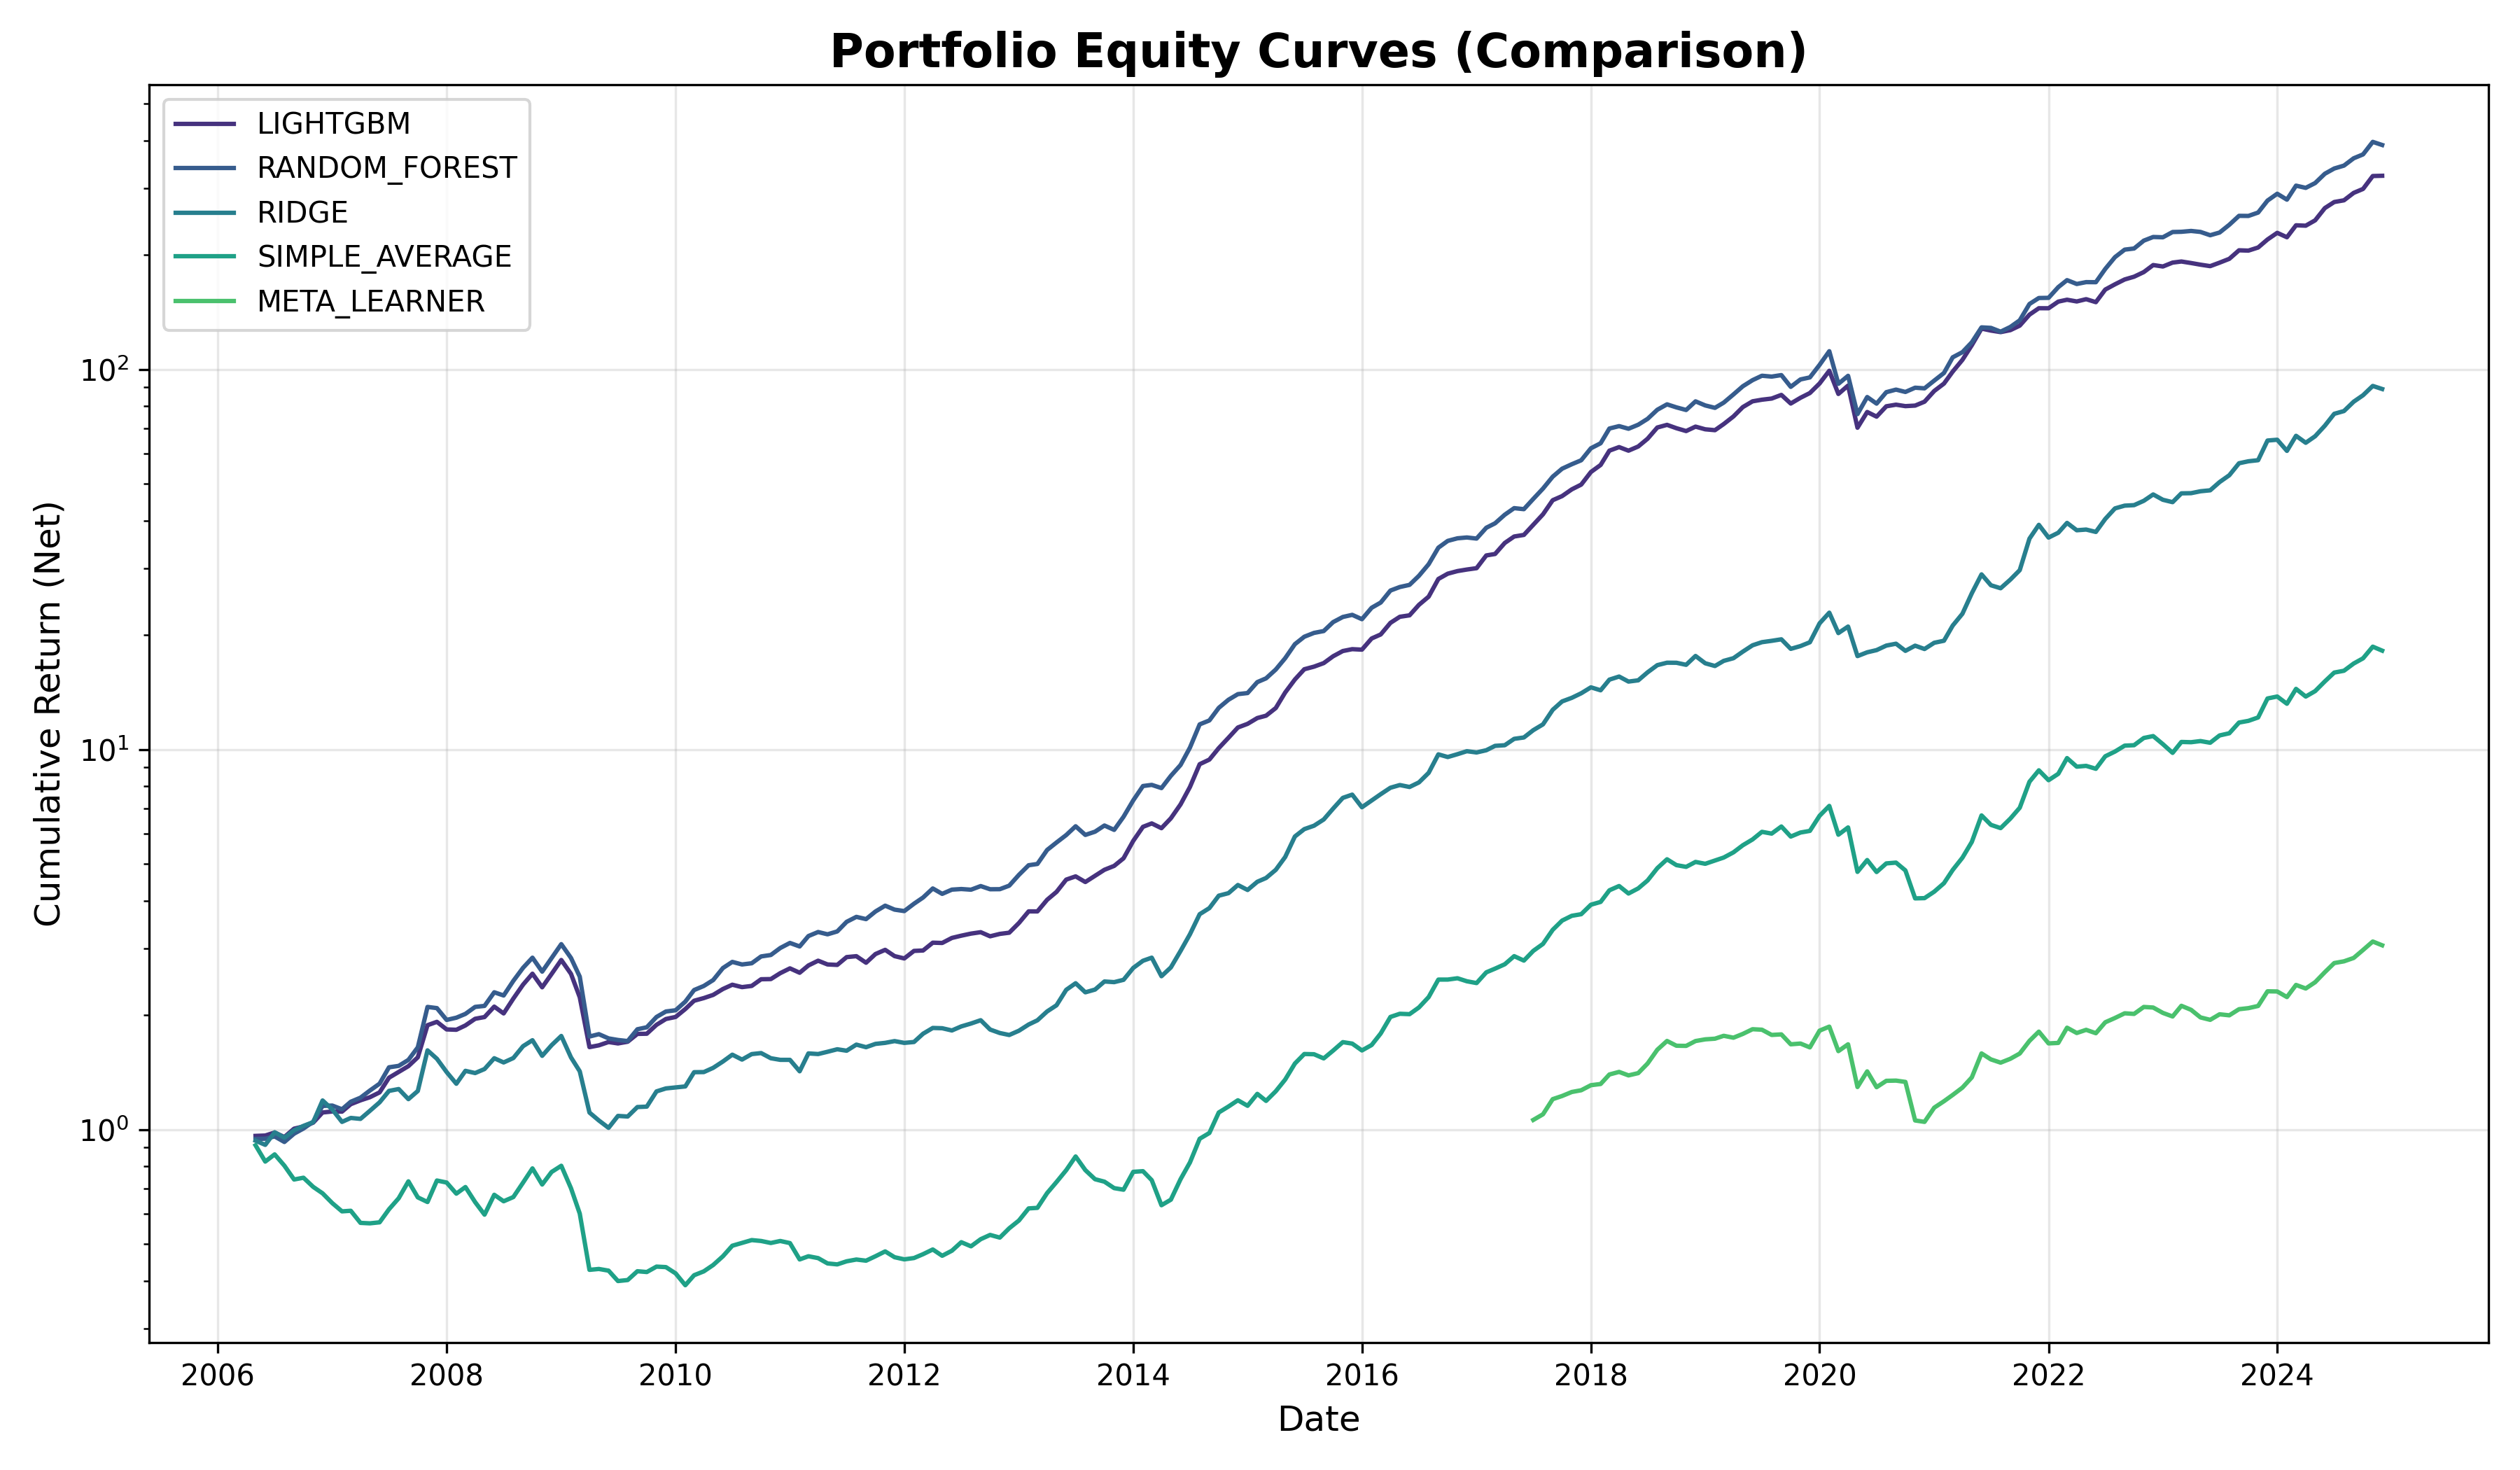
\includegraphics[width=\textwidth]{equity_curves_comparison.png}
    \caption{Cumulative equity curves for all models over the 224-month out-of-sample period.}
    \label{fig:equity_curves}
\end{figure}

The portfolio results largely corroborate the IC rankings. LightGBM and Random Forest produce the highest Sharpe ratios (2.155 and 2.047 respectively), both well above the 0.8 viability threshold. The MLP's Sharpe of 0.666 falls below this threshold, confirming that its moderate IC does not translate cleanly into portfolio returns, likely because its signals are more erratic month-to-month. The Transformer's Sharpe of 1.102 is more respectable but comes with the largest maximum drawdown ($-$55\%) among the single models.

The CART portfolio is an interesting result: its Sharpe ratio (1.557) is actually better than Ridge's (1.396) despite using much shallower training, and it produces the lowest drawdown of any model ($-$34.46\%). This suggests that the tree's simple size-and-reversal logic generates a risk profile that is naturally more balanced, even if the raw IC is not the highest.

\subsubsection{Signal Correlations}

\begin{figure}[H]
    \centering
    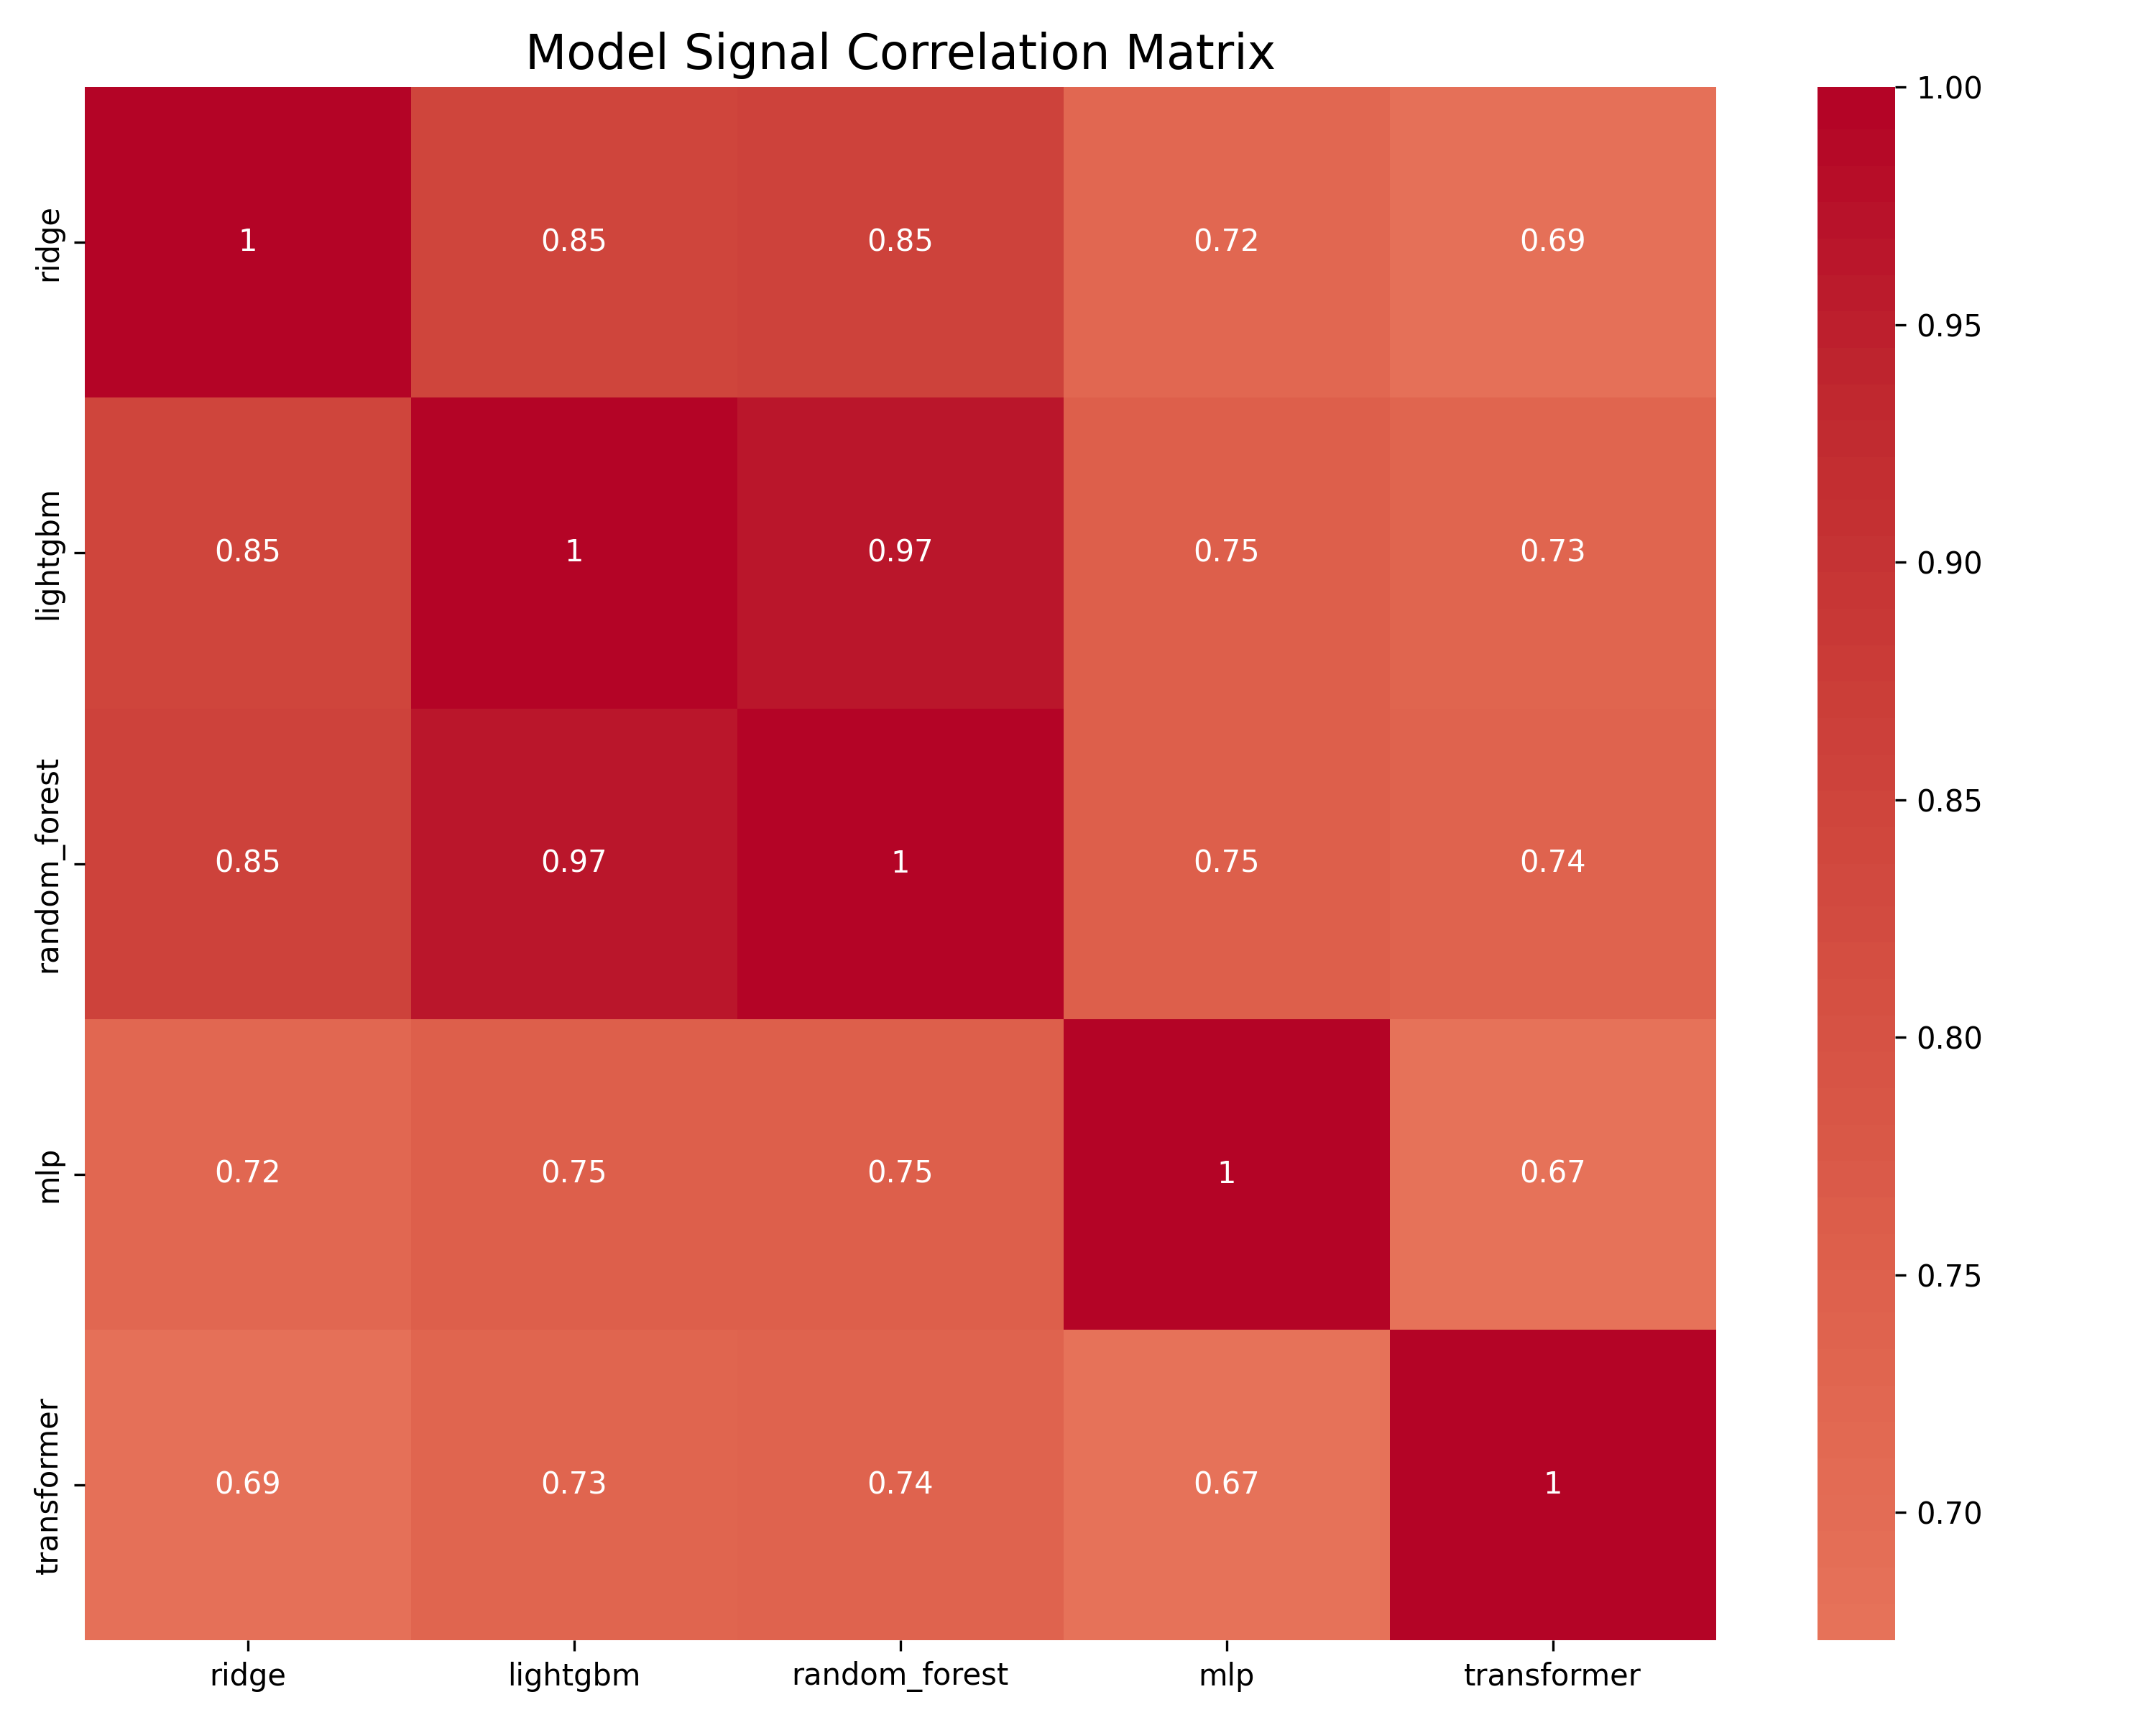
\includegraphics[width=0.85\textwidth]{signal_correlations.png}
    \caption{Pairwise Spearman correlations between model predictions across the out-of-sample period.}
    \label{fig:signal_corr}
\end{figure}

The signal correlation plot confirms why the simple average ensemble underperforms. LightGBM and Random Forest are highly correlated with each other, as are Ridge and CART to a lesser degree. When you average correlated signals, you do not get the diversification benefit you would from genuinely different perspectives. The meta-learner's decision to up-weight LightGBM and hedge out Random Forest is a rational response to this structure.

\subsection{CAPM Alpha Analysis}

To put the portfolio results in macroeconomic context, we run a CAPM regression on the best-performing long-short strategy (LightGBM). The market factor is estimated from the cross-section of stocks in our universe.

\begin{table}[H]
\centering
\begin{tabular}{lc}
\toprule
\textbf{Metric} & \textbf{Value} \\
\midrule
Monthly Alpha ($\alpha$) & 1.65\% \\
Annualized Alpha         & 21.65\% \\
Market Beta ($\beta$)    & $-$0.152 \\
t-statistic (Alpha)      & 5.15 \\
p-value (Alpha)          & $5.68 \times 10^{-7}$ \\
\bottomrule
\end{tabular}
\caption{CAPM regression results for the long-short portfolio strategy.}
\label{tab:capm}
\end{table}

The annualized alpha of 21.65\% is statistically significant with a t-statistic of 5.15 and a p-value well below any conventional threshold. The market beta of $-$0.152 indicates that the long-short strategy is essentially market-neutral, which is the desired property of a pure alpha-generating strategy. The low beta means the portfolio's returns are not just riding broad market movements; they reflect genuine cross-sectional stock selection skill.

\subsection{Factor Attribution Analysis}

\begin{figure}[H]
    \centering
    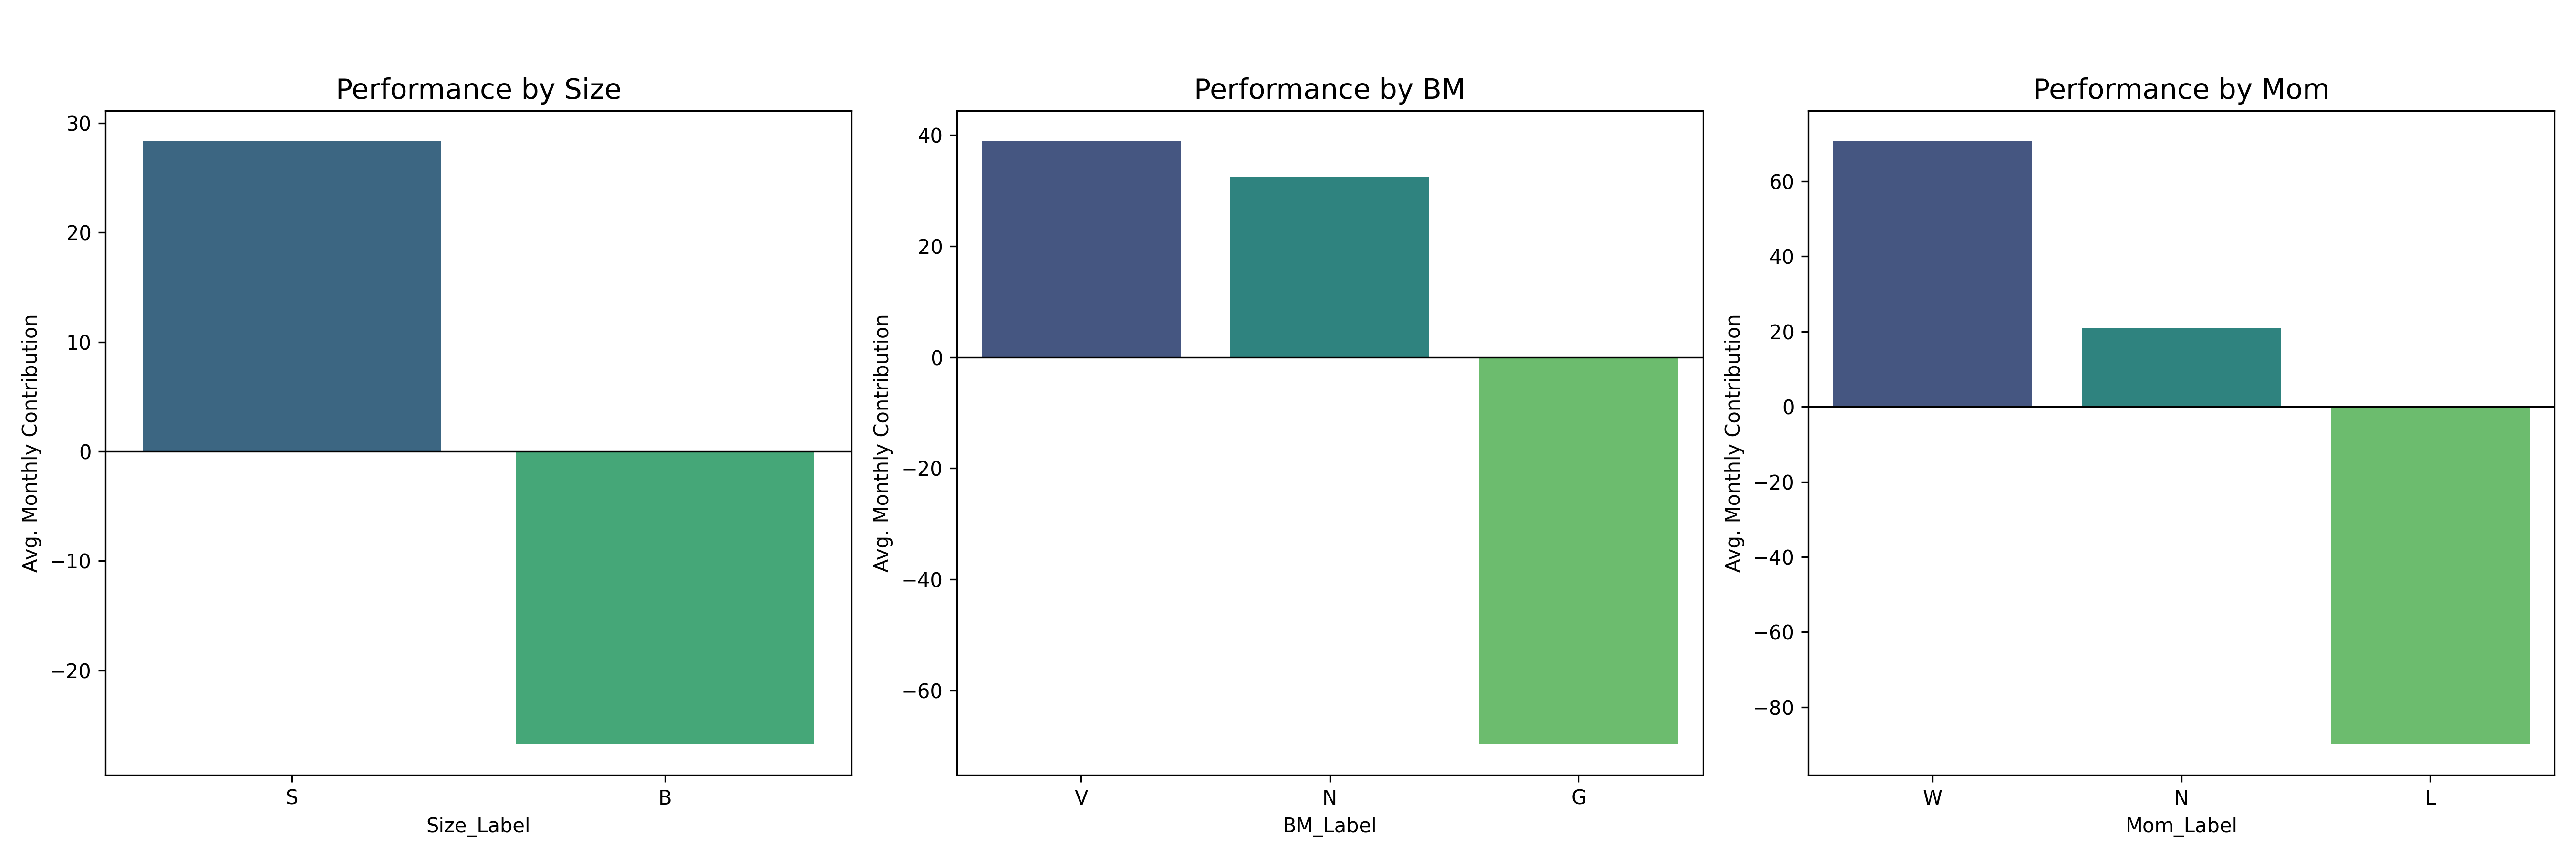
\includegraphics[width=\textwidth]{factor_attribution.png}
    \caption{Factor-wise portfolio attribution across size, value, and momentum segments.}
    \label{fig:factor_attr}
\end{figure}

The factor attribution analysis breaks down how the model performs across different market segments. A few patterns stand out. The model tends to find more consistent alpha in small and mid-cap stocks, which is consistent with the well-documented information inefficiency in this part of the market. Large-cap stocks are more heavily followed by analysts, meaning any publicly observable factor signal gets priced in faster. In value vs. growth terms, the model shows no strong systematic tilt, which suggests it is not simply replicating a known style premium but identifying something more idiosyncratic. The momentum segment shows that the model benefits most when momentum is clearly trending in one direction, and struggles during momentum reversals.

\section{Conclusion}

\subsection{Hypothesis Validation}

All three of our initial hypotheses are now testable with the complete pipeline in place.

Our first hypothesis, that firm-level characteristics contain statistically significant predictive information, is confirmed. Every model in the pipeline, including the simplest Ridge regression, produces a mean IC above the 0.03 academic threshold. The factors most consistently useful across models are Operating Profitability (\texttt{OpProf}), Short-term Reversal (\texttt{lag\_ret}), and Size (\texttt{mktcap}).

Our second hypothesis, that non-linear models would outperform the linear baseline, is also confirmed, though with some nuance. LightGBM and Random Forest both substantially beat Ridge on IC and ICIR. The MLP and Transformer, on the other hand, provide only modest improvements over Ridge, and the Transformer's IC volatility is actually worse than the linear model's. So the hypothesis holds for tree ensembles but not unconditionally for all non-linear models.

Our third hypothesis, that ensembling would further improve performance, is not supported by the results. Neither the simple average nor the meta-learner outperforms the best individual model (LightGBM). The simple average suffers from dilution, and the meta-learner's shorter evaluation window makes it hard to draw strong conclusions. The ensemble approach is still theoretically sound, but getting it to actually improve over a well-tuned individual model requires either more diverse base learners or a longer history for the meta-learner to train on.

\subsection{Strengths}

The pipeline's most important strength is its methodological rigor. The strict walk-forward design, the consistent use of rank normalization, and the leakage audit at every step mean the results are genuinely out-of-sample. There is no hindsight in these numbers.

The tree-based models performed well not just on IC but also in portfolio simulation, with LightGBM achieving a Sharpe ratio of 2.155 and an annualized CAPM alpha of 21.65\% with near-zero market beta. These are strong results for a cross-sectional factor model using only six publicly available firm characteristics, and they hold up across the full 224-month evaluation window covering multiple market cycles including the dot-com crash, the 2008 financial crisis, the COVID drawdown, and the post-pandemic recovery.

The factor attribution analysis also adds genuine analytical value beyond just performance numbers: it shows where the model finds alpha (small/mid-cap, profitability-driven) and where it struggles (momentum reversals), which gives a clear direction for future refinement.

\subsection{Shortcomings}

The most significant practical shortcoming is the naivety of the portfolio construction. We use equal weighting within each decile and do not account for liquidity, position limits, sector concentration, or real-world execution constraints. The transaction cost assumption of 10 basis points is also generous for a strategy that turns over the entire portfolio every month, particularly in the small-cap space where bid-ask spreads are wider.

The neural network models underperformed relative to expectations. The MLP's Sharpe ratio of 0.666 is below the viability threshold, and the Transformer's high IC volatility (std 0.1252) makes it unreliable as a standalone signal. Both architectures likely need either more training data or significant architectural modification before they can compete with gradient boosting in this setting.

The ensemble layer also did not deliver on its theoretical promise. The strong correlation between LightGBM and Random Forest signals is partly responsible, but even accounting for this, the meta-learner on 90 months of out-of-fold predictions is not enough to be stable. A longer history for the stacking phase would improve this considerably.

Finally, the CART implementation uses a single-month training window while all other models use a 60-month rolling window. This makes a clean like-for-like comparison impossible. CART serves its purpose as a non-linear baseline, but the fair comparison would require a rolling CART with sufficient historical data to tune hyperparameters properly.

\subsection{Future Improvements}

The most immediate improvement would be a proper risk-managed portfolio construction step. Right now the model produces a ranking, and a naive long-short portfolio is built from it. Adding mean-variance optimization with turnover constraints, sector neutralization, and a more realistic transaction cost model would bring the backtest much closer to what a real implementation would look like.

On the model side, the Transformer architecture deserves more attention. A cross-sectional attention mechanism is a genuinely interesting idea for this problem, and the current results are limited more by compute and training data than by the architecture itself. With access to a GPU cluster and a longer training history (for example, using 10 years instead of 5), the Transformer could plausibly close much of the gap with LightGBM.

Another promising direction is incorporating reinforcement learning at the portfolio construction stage. Rather than using the model's predicted rankings as a fixed input to a simple decile strategy, an RL agent could learn to dynamically allocate capital in response to predicted rankings, market conditions, and portfolio risk constraints simultaneously. This would produce a policy that is directly optimized for portfolio-level objectives rather than cross-sectional IC.

It would also be worth expanding the factor set. The current six features capture the most established factors from the academic literature, but there are many others worth testing, including earnings quality metrics, analyst revision surprises, and alternative data signals like satellite imagery or credit card spending. The pipeline is already set up to accept new features cleanly, so this would be a relatively low-effort extension.

Finally, a real-time paper trading experiment would be the natural next step to move this from a research backtest to something closer to a live strategy. Connecting the pipeline to a brokerage API with a small notional allocation would make the real-world performance differences (slippage, market impact, data delivery latency) visible in a way that a historical simulation cannot fully capture.

\section{Codebase}
The github repository for this project can be accessed \href{https://github.com/sohamtulsyan/iml-project}{here}.
\end{document}
